
% \addbibresource{./references.bib}

This section we will mainly discuss our measurement about memory performance on the target machine. More specifically, we will report measurements about access latency on each level of memory hierarchy, the memory bandwidth, and the overhead of page fault handling.

\subsection{Memory Latency}

\subsubsection{Methodology}

When measuring access latency on each level of memory hierarchy, basically we followed the method suggest by lmbench\cite{mcvoy1996lmbench}.

We create a linklist which only contains a pointer to the next element:

\begin{lstlisting}
    struct Linklist {
        struct Linklist * next;
    };

    typedef struct Linklist Linklist;
\end{lstlisting}

The total size of the linklist will increase from 1 KB to 256 MB, by the factor of 2. When initializing, a stride will be provided by the tester. The number of the elements in the linklist is always divisible by the stride, and when initializing, the linklist will be decided as many chunks contains stride elements, and each element in one chunk will point to a random element in the next chunk, and the last chunk in the linklist element array will point to the first chunk, which make this linklist an infinite cyclical linklist. This structure will eliminate the impact of cache prefetch, as the stride and random elements can easily make the next element in the linklist out of the prefetch range of each level of cache.

When performing the measurement, in order to get rid of all other unnecessary memory access, we have to use at least \textbf{O1} optimization; however, \textbf{O1} optimization will also optimized the code accessing the linklist. In our final measurement code, the travel of the linklist if write in inline assembly which can avoid compiler optimizations:

\begin{lstlisting}[language=C]
    START_COUNT(high, low);
    while (step --> 0) {
#define INST "movq	(%%rax), %%rax\n\t"
        asm volatile ("mov %0, %%rax\n\t" \
                       HUNDRED(INST) \
                       "mov %%rax, %1"
                       : "=r" (iter)
                       : "r" (iter)
                       : "%rax");
    }
    STOP_COUNT(high1, low1);
\end{lstlisting}

where iter is the head of the linklist. We will measure 100 times of accessing memory on each measurement, and totally perform 1000 (stored in \textbf{step}) measurements.

\subsubsection{Estimation and Results}

\begin{figure}[ht]
    \centering
    \frame{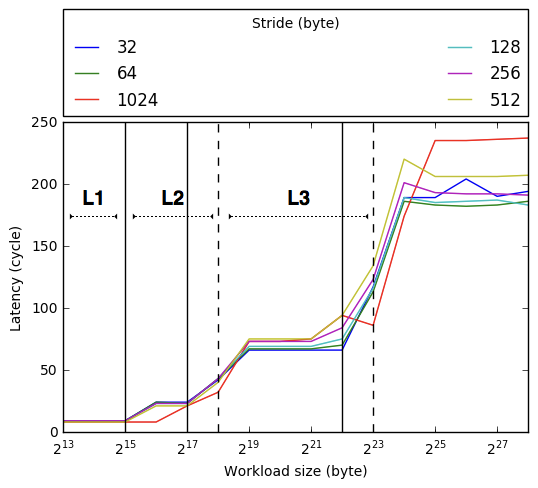
\includegraphics[width = .9\textwidth]{pictures/memLatency.png}}
    \caption{Memory Hierarchy Latency: Estimation and Experiment Results }
    \label{mem_latency_result}
\end{figure}

\begin{table}[ht]
  \centering
  \caption{\textbf{Memory hierarchy Latency: Estimation and Experiment Results}}
  \begin{threeparttable}
  \begin{tabular}{ccc}
  \hline
      \textbf{Memory}    & \textbf{Latency}   & \textbf{Expr. Results} \\
      \textbf{Hierarchy}   & \textbf{Estimation}  & (AVG)   \\
  \hline
      \textbf{L1}  & 5 cycles (1.79 ns) & 9 cycles (3.22 ns)   \\
      \textbf{L2}  & 20 cycles (7.16 ns) & 20 cycles (7.16 ns)  \\
      \textbf{L3}  & 60 cycles (21.48 ns) & 70 cycles (25.06 ns)  \\
      \textbf{Memory}  & 150 cycles (53.70 ns)  & 190 cycles (68.02 ns)  \\
  \hline
  \end{tabular}
  \end{threeparttable}
  \label{memory_latency_table}
\end{table}

For estimation, we believe the latency for l1 cache references should be pretty low, let's say, within 5 cycles; the latency for l2 cache should be higher, let's say, 20 cycles; the latency for l3 cache should be much higher than l2, let's say, 60 cycles; and the latency for main memory should be the highest and much higher than l3 cache, let's say, 150 cycles.

The result is shown in \textbf{Figure \ref{mem_latency_result}} and \textbf{Table \ref{memory_latency_table}}. In \textbf{Figure \ref{mem_latency_result}}, the real lines separate the latency turning point for different level of memory hierarchy, and the dotted lines separate the real size of different levels of the memory hierarchy on the target machine. As we can see in the figure, the dotted line and the real line for l1 cache is in the same position, but for l2 cache and l3 cache, the latency turning point is always a little bit smaller than the actual size point. For why that happened, we guess that the following reason contributes it: as both l2 and l3 cache are unified instruction and data cache, so that some instructions stored in the l2 cache and l3 cache will accelerate that data access latency turning point to happen.

\textbf{Table \ref{memory_latency_table}} shows the latency estimation and measurement results. We under estimate the access latency of l1 cache and memory.

\subsection{Memory Bandwidth}
\label{sec:memorybandwidth}
\subsubsection{Methodology}

When measuring memory bandwidth, we use the method metioned in \cite{mcvoy1996lmbench}, which is using integer reading and writing which miss at l3 cache to measure the reading and writing bandwidth for main memory. However, there are several technical details not mentioned in \cite{mcvoy1996lmbench} we need to point out here.

First, although we are reading and writing 4 Byte integers when running the measuring code, to calculate memory bandwidth, we need to use 64 Byte as the size for each memory access, as when transferring data back and forth between main memory and l3 cache, data is always transferred with a l3 cache line size. The l3 cache line size can be retrieved by the command:

\begin{lstlisting}
    cat /sys/devices/system/cpu/cpu0/cache/index3/coherency_line_size
\end{lstlisting}

At the same time, in order to get rid of cache line prefetch, we need to accessing data with a stride at least as large as the l3 cache line size. In our experiments, we use 256 byte (or 64 integers) as an accessing stride.

Furthermore, by using the command:

\begin{lstlisting}
    sudo lshw -C memory
\end{lstlisting}

we can retrieve the writing policies for each level cache. In our experiment computer, l1 and l2 cache are both write-through cache, while l3 cache is an internal write-back unified cache. Although it does not mention the write miss policy, \cite{wiki:cache} indicates that write back policy usually pairs with write allocation policy. Due to these facts, there is some details in the implementation:

\begin{enumerate}
    \item In order to get rid of caching effect of l3 cache, we first fill l3 cache with data that will never be read and write during measurement process.
    \item When measuring reading bandwidth, we need to fill l3 cache with clean cache lines, orderwise when we reading the measurement data from main memory to l3 cache, there will be a high dirty block writing back overhead when evicting cache lines.
    \item When measuring writing bandwidth, we want all measurement data to experience a write miss. However, l3 cache itself is write-allocation, thus even a write miss will not write back to main memory. In this case, the way we solve this problem is filling all l3 cache line with dirty cache data before we start measurement. As a result, each time we write a measurement writing data, as l3 cache is a write allocation cache with full of dirty data, so that each time l3 cache will evict a dirty line as each time we are accessing different l3 cache set, which means that each time we write, we will finally write a dirty cache line back to main memory, and thus we can measure the memory writing bandwidth.
\end{enumerate}

\subsubsection{Estimation and Results}
\label{Memory_bandwidth_result_section}

\begin{table}[ht]
  \centering
  \caption{\textbf{Memory Bandwidth: Estimation and Experiment Results}}
  \begin{threeparttable}
  \begin{tabular}{ccccc}
  \hline
      \textbf{Read or} & \textbf{Bandwidth}   & \textbf{Expr. Results} & \textbf{Standard}\\
      \textbf{Write}   & \textbf{Estimation}  & (AVG)   & \textbf{Deviation} \\
  \hline
      \textbf{Read}  & 10600 MB/s & 7131.15239595 MB/s & 394.490122927  \\
      \textbf{Write} & 10600 MB/s & 6709.49876645 MB/s & 1191.12060254  \\
  \hline
  \end{tabular}
  \end{threeparttable}
  \label{memory_bandwidth_table}
\end{table}

For estimation, Frank Denneman stated on his web blog \cite{frankdenneman} that, the bandwidth for both reading and writing of a DDR3-1333 memory is 10600 MB/s, we take this as our estimation.

The measurement result is shown in \textbf{Table \ref{memory_bandwidth_table}}. The results show that memory reading bandwidth should be \textbf{7131.15239595 MB/s}, and writing bandwidth should be \textbf{6709.49876645 MB/s}. The measurement result is below the estimation value, we think the reason for that is:

First, in this experiments, under our accessing pattern, it is hard for main memory to achieve its theoretical optimized reading and writing speed, as the bank row cache inside the DRAM will miss, thus an entire row and column retrieve process is needed each time we accessing;

Second, the software overhead is unavoidable, this will also decrease our memory performance.

The writing bandwidth is smaller than reading bandwidth, as \textbf{Table \ref{memory_bandwidth_table}} shown. This is reasonable, as writing do be slower than reading in DRAM.

\subsection{Page Fault Handling}

\subsubsection{Methodology}

When measuring page fault handling overhead, we will first create a large file (40 MB) on disk, then use \textbf{mmap()} system call, to map the file into the main memory. Then, we will read data in that file, as \textbf{mmap()} only mapping that file into destination memory chunks, not reading file contents into main memory, the reading operation will cause a page fault. The operating system will handle that page fault, and that's what we want to measure.

There is still one problem needs to be addressed out, the file system optimization. The file system will cache the contents of the file and also perform file prefetch from the disk, so that, if we failed to bypass those optimization, we could not accurately measure the page fault handling overhead. To bypass that optimization, the measurement program will access the file with a stride applied with a random offset on page.

We used to create a 150 MB file in /tmp directory for mapping, however, it turns out that the overhead for handling page faults after mapping in this file is significantly smaller than a HDD's overhead, and there is no seek penalty exist, and obviously this file is actually stored in memory. In the second round, we changed the directory for the temporary mapping file to the current directory of the benchmark binary, the expanded the file size to 16 GB, after that, we can observe seek penalty now.

\subsubsection{Estimation and Results}

\begin{table}[ht]
  \centering
  \caption{\textbf{Pagefault Handling Overhead: Estimation and Experiment Results}}
  \hspace*{-3em}\begin{threeparttable}
  \begin{tabular}{cccccc}
  \hline
        \textbf{HW Overhead} & \textbf{SW Overhead } & \textbf{Total Overhead} & \textbf{Expr. Results} & \textbf{Standard}\\
        \textbf{Estimation}       &  \textbf{Estimation}         & \textbf{Estimation}  & (AVG)   & \textbf{Deviation} \\
  \hline
        28000000 cycles & 10000 cycles & 28010000 cycles (10.03 ms)  & 22672005.8858 cycles (8.12 ms) & 7299383.2799 \\
  \hline
  \end{tabular}
  \end{threeparttable}
  \label{pagefault_handle_time}
\end{table}

For estimation, the I/O speed of a 7200 RPM HDD is at the scale of 100 MB/s \cite{wiki:hdd}, so that transferring a 4K page will take:

$$ \frac{4KB}{100 MB/s} = \frac{1}{25600} s $$

$\frac{1}{25600} s$ equals to around $111600 cycles$.

In checkpoint 2 we made a mistake: we ignored that in a HDD environment, seek and rotation is the most significant overhead for page fault handling, when taking in consider about seek and rotation, the time consumption is of the order of 10 ms. So that, the hardware overhead should be:

$$\frac{10 ms}{0.350001 ns/cycle} = 27932882 cycles$$

So the total hardware overhead should be around $28000000 cycles$

The software overhead mainly comes from page table maintains and protection mechanism, and we assume this overhead is around 10000 cycles. Then, the total estimation overhead for a page fault handling is 28010000 cycles.

The result is shown in \textbf{Table \ref{pagefault_handle_time}}. We underestimate the overhead of the page fault handling by around 2 ms. As there is a high variance for the performance of the disk, it is not strange that this difference exist. It will not experience the largest disk access overhead for each access request.

The result is shown in \textbf{Table \ref{pagefault_handle_time}}. The speed is a little bit faster than what we estimate, this should be caused by each time a page fault happened, the disk seeking and rotation overhead is not always as high as 10 ms.

For the question about speed compare between memory bandwidth and page fault page transfer bandwidth on byte scale, according to \textbf{Section \ref{Memory_bandwidth_result_section}}, on average the memory can transfer a byte in

$$\frac{1 Byte}{7131.15239595 MB/s} = 0.133734 ns $$

and the page fault mechanism can transfer a byte in

$$\frac{1 Byte}{\frac{4 KB}{8.12 ms}} = 1982.421875 ns $$.

Thus the page fault handling is around 15000X more expensive than a page hit memory access.
